%!TEX root = thesis.tex

\chapter{Cryptographic Primitives}
Secure computation is a cryptographic technique for securely computing a function between two parties.
We split secure computation into two cases: cases where there are two parties involved, referred to as two-party computation (2PC), and cases where there are three or more parties, referred to as multiparty computation (MPC).
This thesis focuses on 2PC protocols, but many of the methods are applicable to MPC as well.

2PC protocols are complex cryptographic protocols that rely on a number of cryptographic primitives.
In order to understand 2PC, it is not crucial to understand how the cryptographic primitives work, but it is important to understand their inputs, outputs and security guarantees. 
This first chapter will give an overview of the cryptographic primitives used in 2PC protocols.

\section{Introducing Cryptographic Security} 
The goal of this section is to explain cryptographic security, starting at an intuitive level and moving into more complex ideas. 
We do not present cryptographic security in a comprehensive fashion; rather, we explain cryptographic security with the goal of explaining 2PC protocols and their security.
For more information on cryptographic security, we encourage the reader to peruse \cite{katzlindelltextbook}. 

We define a few intuitive terms to get started.
A \textit{cryptographic scheme} is a series of instructions designed to perform a specific task. 
An \textit{adversary} is an algorithm that tries to \textit{break} the scheme. 
If an adversary \textit{breaks} a scheme, then the adversary has learned information about inputs to the scheme that they shouldn't. 

One aim of defining security in cryptography is to build a formal definition that matches real world needs and intuitions. 
A good starting place is to consider perfect security. 
A scheme is perfectly secure if no matter what the adversary does, they cannot break the scheme.
Even if the adversary has unlimited computational power, in terms of time and space, an adversary cannot break a perfectly secure scheme. 

However, perfect security is not the most useful way to think of security, because it forces schemes to be slow and communication-intensive.
We relax the definition of security by requiring that the adversary run in polynomial time. 
This substantially reduces the power of the adversary, and it matches our intuition: we are really only concerned with what adversaries can reasonably achieve, as opposed to what is theoretically possible. 

Because computers have improved drastically over the years, what was previously considered a reasonable adversary is not what is considered a reasonable adversary today. 
Modern computing advances have created easy access to faster computation, meaning that modern adversaries can solve harder problems than they could in previous years. 
As a concrete example, consider giving an adversary the following problem: find the factors of $N$. 
The average computer today can solve the problem for a larger $N$ than the average computer could a decade ago.

The changing computational power highlights the importance of being able to scale how hard it is to break a cryptographic scheme.
To this end, we introduce a \textit{security parameter}, denoted as $\lambda$.
A security parameter is a positive integer that represents how hard a scheme is to break; a larger security parameter should mean that the scheme is more difficult to break. 
More specifically, the security parameter is correlated to the input size of the problem underlying the cryptographic scheme. 
For example, if the underlying problem is factoring a large number $N$, then $\lambda$ is the number of bits needed to express $N$ in binary, that is, $\lambda = |N|$.
As $N$ and $\lambda$ scale up, the factoring problem becomes more difficult and the scheme becomes harder to break. 

Finally, we acknowledge that adversaries have access to some random values, hence we strengthen adversaries to be probabilistic algorithms. 
Probabilistic means that the algorithms have access to a string of uniform random bits, with the implication being that the algorithm is capable of guessing. 

In order to reason about the security of cryptographic schemes, it is useful to think about breaking a scheme in terms of a probability. 
For example, we want to be able to say that the best adversary, that is best probabilistic polynomial-time algorithm, has some probability $p$ of breaking the scheme. 
We note that $p$ is nonzero, since the adversary can always guess and be right with some nonzero probability. 
To achieve a probability based formalism, we introduce a negligible function.
Informally, a negligible function is smaller than the reciprocal of all polynomial functions.

\begin{definition}
\label{defn:negible}
A function $\mu : \NN \to \RR$ is negligible if for all positive polynomial $p(\cdot)$, there exists positive integer $N_p$ such that for all $x > N_p$, 
\begin{equation}
    |\mu(x)| < \frac{1}{p(x)}.
\end{equation}
\cite{goldreich}
\end{definition}

Examples of negligible functions include $2^{-n}$, $2^{- \sqrt{2}}$ and $n^{- \log n}$. 

To put a negligible function to use, say an adversary is attacking a cryptographic scheme that is equivalent to solving a problem $P$ with input size $\lambda$ and $2^{\lambda}$ possible answers. 
Moreover, say that $P$ is known to be NP-hard such that there is no polynomial time algorithm to solve $P$. 
Then, the best that the adversary can do might be to guess the answer to $P$.
Hence the probability that the adversary successfully answers $P$, or breaks the scheme, is 
\begin{align*}
Pr[\text{A correctly answers $P$}] & = {2^{- \lambda}}
\end{align*}
Since $2^{- \lambda}$ is a negligible function, we say that the adversary has a negligible probability of breaking the scheme. 

In summary, we model an adversary as a probabilistic polynomial-time algorithm. 
This limits the computational power of the adversary to what is reasonably computable in reality. 
Moreover, we can scale the security of a scheme or problem by changing $\lambda$, the security parameter, where a higher security parameter makes the scheme more difficult to break. 

\section{Encryption}

Encryption is the process of obfuscating a message, and then later un-obfuscating the message.
Say Alice has a message that she wants to send to Bob, but somewhere between Alice and Bob sits Eve, who wants to learn about the message.
An encryption scheme enables Alice to send her message to Bob with confidence that Eve cannot learn any information about the message. 

An encryption scheme is composed of three algorithms: $\Enc$, $\EncInv$ and $\Gen$; formally, we say an encryption scheme is a tuple $\Pi = (\Gen, \Enc, \EncInv)$.\footnote{We use $\Pi$ here to denote the encryption scheme, because it is a protocol. Protocol starts with a p.}
$\Enc$ the obfuscating algorithm, $\EncInv$ is the un-obfuscating algorithm and $\Gen$ generates a key. 
The key is extra information that $\Enc$ and $\EncInv$ use to obfuscate and un-obfuscate the message respectively. 
The key, denoted $k$, is a random\footnote{The notion of randomness in cryptography is precisely defined, and in cases where $\lambda$ is large, it is sufficient for $k$ to be pseudorandom. Pseudorandomness is also precisely defined.} string of $\lambda$ bits, that is $k$ is randomly sampled from the set $\{0,1\}^{\lambda}$  where $\lambda$ is the security parameter of the encryption scheme. 
As per the discussion on security parameters, as $\lambda$ increases and $k$ grows in length, the encryption scheme should become harder to break.

$\Enc$, the encryption algorithm, takes a message and the key as input and outputs an obfuscated message. 
$\EncInv$, the decryption algorithm, takes the encrypted message and the key as input and outputs the original message. 
We refer to the original message as the plaintext or $pt$ and the encrypted message as the ciphertext or $ct$. 

\begin{equation}
    \label{eqn:encryption}
    \begin{split}
    	\Gen(1^n) & \rightarrow k \\
        \Enc_k (pt) & \rightarrow ct  \\
        \EncInv_k(ct) & \rightarrow pt
    \end{split}
\end{equation}

We are not concerned with how encryption schemes are implemented or on what problems they rely; rather, we use encryption schemes as subroutines, so we are concerned with the security guarantees that they offer.

We define security using a thought experiment. 
In the thought experiment, the adversary has access to the encryption algorithm with the key hardcoded in. 
This means that the adversary can encrypt any message they want, and see how the message would encrypt. 
The goal of the adversary at this point in the thought experiment is to find a pattern or weakness in the encryption algorithm that they can exploit.
The adversary eventually picks any two messages $m_0$ and $m_1$; the adversary shows us $m_0$ and $m_1$.
We choose one of the messages\footnote{We select the message uniformly at random.}, encrypt the message, and send the resulting ciphertext to the adversary.
The adversary's goal now is to determine which message we encrypted.
They still may use their encryption algorithm with the key hardcoded.
Eventually the adversary must output either $0$ or $1$ indicating that they think we selected $m_0$ or $m_1$ to encrypt, respectively.
If the adversary picks correctly, then we say that the adversary wins; otherwise, we say that the adversary loses.
We consider the encryption scheme to be secure if the probability that the adversary wins is $\frac{1}{2} + \mu(\lambda)$ where $\mu$ is a negligible function, i.e. the best the adversary can do is guess.

\begin{definition}
An encryption scheme is secure under a chosen-plaintext attack if for all probabilistic polynomial-time adversaries $A$, there exist a negligible function $\mu$ such that
\begin{equation}
Pr[E_{\A, \Pi}(n) = 1] \leq \frac{1}{2} + \mu(n)
\end{equation}
where $E$ is the following experiment:
\begin{enumerate}
\item Generate key $k$ by running $\Gen(1^n)$. 
\item The adversary $\A$ is given $1^n$ and oracle access to $\Enc_k$, and outputs a pair of messages $m_0$ and $m_1$ of the same length.
\item A uniform bit $b \samples \{0,1\}$ is sampled uniformly at random, and then ciphertext $c \gets \Enc_k(m_b)$ is computed and given to $\A$.\footnote{Throughout this thesis, we use the notation $x \samples X$ to mean that x is sampled uniformly at random from the set $X$. We use the arrow $\gets$ to indicate that a value to being assigned to variable. For example, $x \gets 3$, means that $x$ is being assigned the value $3$.}
\item $\A$ continues to have oracle access to $\Enc_k$, and outputs a bit $b'$. 
\item The output of the experiment is defined to be $1$ if $b' = b$ and $0$ otherwise. If at any point $\A$ encrypts $m_0$ or $m_1$ with their encryption oracle, the output is $0$. $1$ indicates that the adversary wins, and $0$ indicates that the adversary loses.
\end{enumerate}
\end{definition}

It is useful for 2PC to create an encryption scheme that requires two keys to encryption and decrypt.
An encryption scheme with two keys is called a \textit{dual-key cipher} (DKC) \cite{bellare2012foundations}.
It is easy to instantiate a DKC if one has a secure single-key encryption scheme: let $k_0$ and $k_1$ be two keys and instantiate the DKC as follows:
\begin{equation}
    \begin{split}
        \EncDKC_{k_0, k_1}(pt) = \Enc_{k_1} ( \Enc_{k_0} ( pt )) \\
        \EncDKCInv_{k_0, k_1}(ct) = \EncInv_{k_0} ( \EncInv_{k_1} ( ct )) 
    \end{split}
\end{equation}

If the encryption scheme used to create the DKC is secure, then it is easy to see that the DKC is also secure.
We are formally considering the statement: if $\Enc$ is secure then the constructed DKC is secure. 

Consider the contrapositive: if the constructed DKC is insecure then $\Enc$ is insecure. 
We sketch a proof of this claim.
Suppose that we have an adversary $\A$ competing in the $\Enc$ security experiment, and $\A$ can break the DKC security experiment - this assumption is made since we assume that the DKC is insecure.
Since $\A$ can beat the DKC experiment, $\A$ finds two messages, $m_0$ and $m_1$, such that they can determine $b$ given $\Enc_k(\Enc_k(m_b))$.

In the $\Enc$ experiment, $\A$ sets $m'_0 \gets \Enc_k(m_0)$ and $m_1' \gets \Enc_k(m_1)$ using their encryption oracle.
The adversary submits $m_0'$ and $m_1'$ as their messages, and they recieve back $\Enc_k(m_b')$.
Since $\Enc_k(m_b')$ is actually $\Enc_k(\Enc_k(m_b))$, the $\A$ can determine $b$.
The adversary can do this because they chose $m_0$ and $m_1$ such that they could beat the DKC security experiment.
Finally, $\A$ outputs $b$, which will be correct with probabilty greater than $\frac{1}{2} + \mu(\lambda)$ where $\mu$ is a negligible function.
Therefore the adversary can break the $\Enc$ experiment if they can break the DKC experiment, and the contrapositive of this statement tells us that if the $\Enc$ scheme is secure, then the DKC scheme is also secure.

\section{Computational Indistinguishability}
This section introduces the idea of computational indistinguishability. 
We do not use computational indistinguishability immediately, but it will important later for defining security of a 2PC protocol.

Informally, two probability distributions are indistinguishable if no probabilistic polynomial-time algorithm can tell them apart.
The thought experiment is like this: an algorithm knows that there are two distributions.
It samples from one of the distributions.
If the algorithm correctly determines which distribution it was given, then it wins, and otherwise the algorithm loses.
The algorithm, since it must run in polynomial time, can only sample a polynomial number of values from the distributions.

Formally, computational indistinguishability is:

\begin{definition}
\label{defn:computational-indistinguishability}
Let $\mathcal{X} = \{X_n\}_{n \in \NN}$ and $\mathcal{Y} = \{Y_n\}_{n \in \NN}$ be distribution ensembles.
$\mathcal{X}$ and $\mathcal{Y}$ are computationally indistinguishable, denoted $\mathcal{X} \compindist \mathcal{Y}$, if for all probabilistic polynomial-time algorithms $D$, there exists a negligible function $\mu$ such that:
\begin{equation}
    |Pr_{x \gets X_n} [D(1^n, x) = 1] - Pr_{y \gets Y_n} [D(1^n, y) = 1]| < \mu(n)
\end{equation}
\cite{katzlindelltextbook}.
\end{definition}

We break down the definition.
The unary input $1^n$ tells the algorithm $D$ to run in polynomial time in $n$.
The probability distributions $X_n$ and $Y_n$ are restricted by $n$, which in this context is the security parameter.
The phrases $x \gets X_n$ and $y \gets Y_n$ mean that the probability is taken over samples from the distributions.

\section{Boolean Circuit} 
A function in a 2PC protocol is represented as a boolean circuit.
A boolean circuit takes as input $x \in \{0,1\}^n$, performs a series of small operations on the inputs, and outputs $y \in \{0,1\}^m$.  
You may have encountered circuits and logical operators in another context, where the inputs and outputs were True and False.
For our usage, True corresponds to the value $1$, and False corresponds to the value $0$. 

The small operations done inside of a circuit are performed by a \emph{gate}.
A gate is composed of three wires: two input wires and one output wire, where a \emph{wire} can have a value either $0$ or $1$.
A gate performs a simple operation on the two inputs, resulting in a single output bit.
Table \ref{tab:xor} gives the mapping of an XOR gate.

\begin{table}[h]
\label{tab:xor}
\centering
\begin{tabular}{ | l | c || r |}
\hline
x & y & xor(x,y) \\ \hline
1 & 1 & 0 \\ \hline
1 & 0 & 1 \\ \hline
0 & 1 & 1 \\ \hline
0 & 0 & 0 \\ \hline
\end{tabular}
\caption{Logical table of XOR gate}
\end{table}

A circuit is a combination of gates that are strung together.
It turns out that circuits are quite powerful: in fact, a circuit composed only of AND gates, XOR gates and NOT gates can compute any function or algorithm \cite{goldreich}.
In other words, if there is some algorithm that can do it, then there is some circuit that can do it as well.

\begin{figure}[h]
    \centering
\begin{circuitikz} \draw
    (0,2) node[and port] {};
\end{circuitikz}
\caption{An AND gate.}
\end{figure}

\begin{figure}[h]
    \centering
\begin{circuitikz} \draw
    (0,2) node[xor port] {};
\end{circuitikz}
\caption{An XOR gate.}
\end{figure}

\begin{figure}[h]
    \centering
\begin{circuitikz} \draw
    (0,2) node[not port] {};
\end{circuitikz}
\caption{A NOT gate.}
\end{figure}

\begin{table}[h!]
\label{tab:less_than}
\centering
\begin{tabular}{ | l | c || r |}
\hline
x & y & $x < y$ \\ \hline
0 & 0 & 0 \\ \hline
0 & 1 & 1 \\ \hline
1 & 0 & 0 \\ \hline
1 & 1 & 0 \\ \hline
\end{tabular}
\caption{Logical table of less than function}
\end{table}

\section{Oblivious Transfer}

\begin{figure}[h]
    \center
    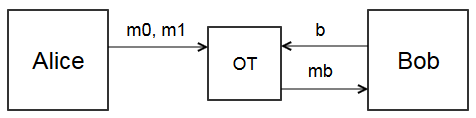
\includegraphics[scale=.8]{images/ot}
    \caption[Overview of oblivious transfer]{The high level idea of oblivious transfer. Image from \cite{alexirpan}}
    \label{fig:basic-ot}
\end{figure}
Oblivious Transfer (OT) is a simple, useful protocol that underlies many more complicated crypto-systems \cite{EGL82, Rab05}.

Figure \ref{fig:basic-ot} outlines the high level idea of oblivious transfer.
The box labeled OT in figure \ref{fig:basic-ot} may be thought of as a trusted post office.
Alice potentially sends two messages $m_0$ and $m_1$ to Bob, but instead of sending the messages to Bob, she sends the messages to the post office.
Bob, without seeing either $m_0$ or $m_1$, knows that he wants $m_b$ where $b \in \{0,1\}$, so he notifies the post office that he wants message $b$.
With this information, the post office gives Bob $m_b$.
We want two secure properties to hold: (1) Alice does not know whether Bob received $m_0$ or $m_1$ and (2) Bob does not learn any information about $m_{1-b}$, the message that he did not receive.

We will not focus on the internal operations of oblivious transfer; for our purposes, it is a secure black box.
When we use oblivious transfer in the next chapter, the two messages that Alice potentially sends will be encryption keys, and Bob will select a key that corresponds to his input - a value that he doesn't want Alice to know.
In Chapter 3 we will discuss improvements to oblivious transfer, since oblivious transfer, despite its simple appearance, is computationally expensive.
